\documentclass[11pt, a4paper]{article}
\usepackage[utf8]{inputenc}
\usepackage{graphicx}
\graphicspath{{./images/}}

\usepackage{hyperref}

\title{Advanced Lane Line Finding}
\author{Samuel Navarro}
\date{\today}

\begin{document}
\maketitle

\tableofcontents{}



\section{Camera Calibration}
\label{sec:camera_calibration}

The code for this step is implemented in the third and fourth cell of the jupyter notebook in the functions \texttt{show\_image} and \texttt{calibrate\_camera}. 

The output of \texttt{calibrate\_camera} gives us the objpoints and the imgpoints arrays. I then use this arrays to obtain the distortion coefficients and the camera matrix to obtain the undistorted image. 

An example is in the Figure 1 and 2~\ref{fig:undistort} 


\begin{figure}[htb!]
    \centering
    \begin{minipage}{0.5\textwidth}
        \centering
		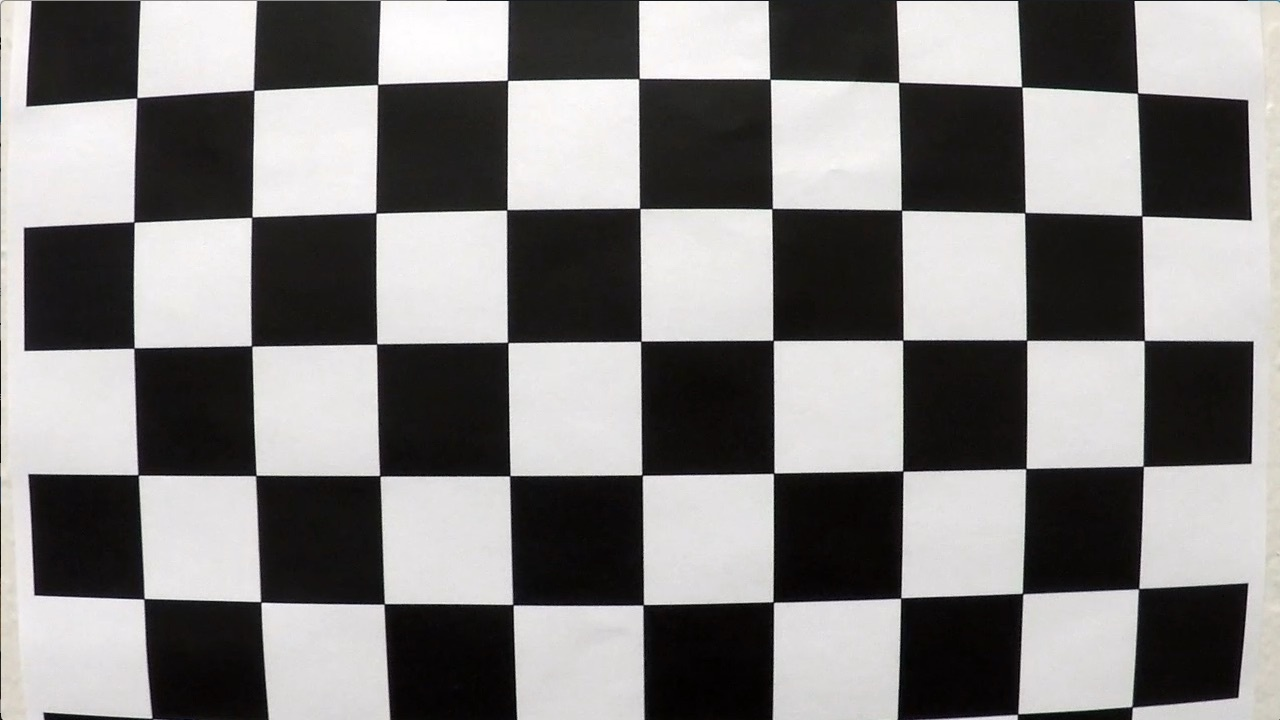
\includegraphics[width=1\textwidth]{chess_img} 
        \caption{Original}
		\label{fig:original_chess}
    \end{minipage}\hfill
    \begin{minipage}{0.5\textwidth}
        \centering
		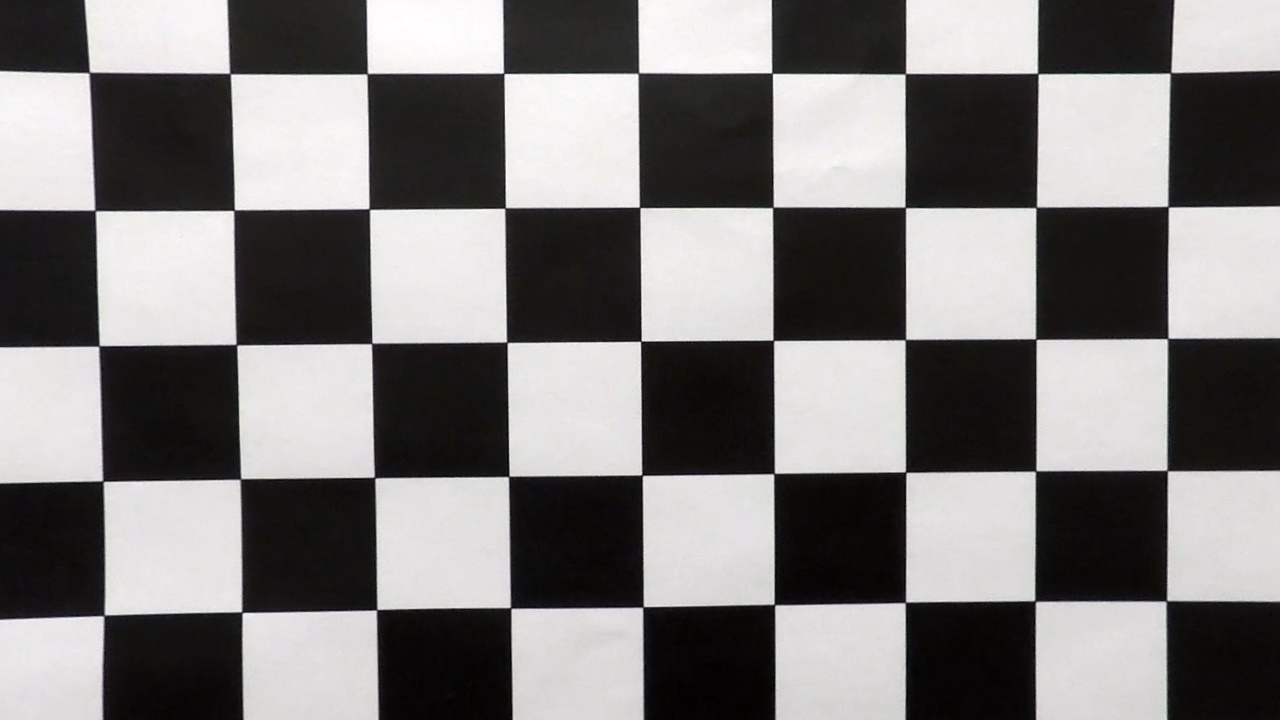
\includegraphics[width=1\textwidth]{undistorted_chess} 
        \caption{Undistorted}
		\label{fig:undistorted_chess}
    \end{minipage}
	\label{fig:undistort}
\end{figure}


\section{Pipeline Images}
\label{sec:pipeline_images}

\subsection{Undistorted test}%
\label{sub:undistorted_test}


We can see the distortion correction being applied in one of the test images:

\begin{figure}[htb!]
	\centering
	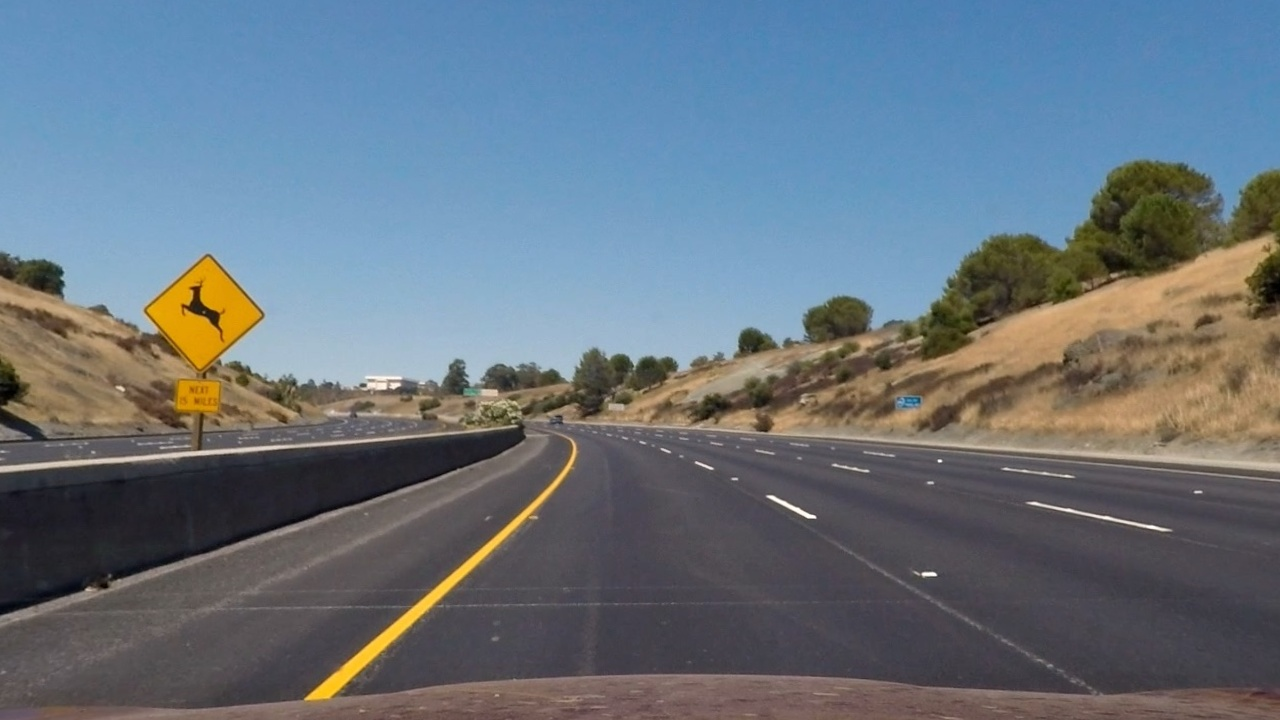
\includegraphics[width=0.8\linewidth]{undist}
	\caption{Undistorted test}
	\label{fig:undistorted_test}
\end{figure}

\subsection{Perspective Transform}%
\label{sub:perspective_transform}

The perspective transform is in the function \texttt{perspective\_transform} in the same notebook.

The parameters I used was hardcoded. This is obviously something that can be improved. The most straightforward way I can think of based on what we've learned is applying Hough Transform in the image and apply the perspective transform on that. 

The result is in the Figure~\ref{fig:warped}:


\begin{figure}[htb!]
	\centering
	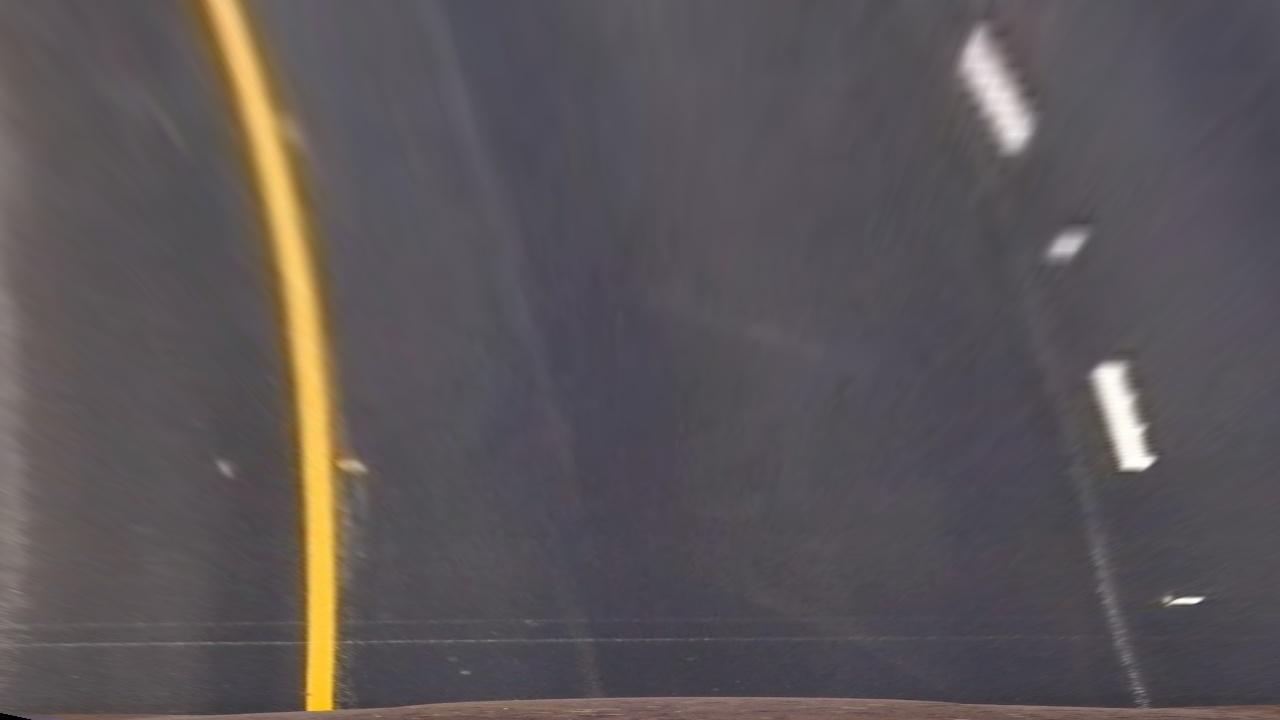
\includegraphics[width=0.8\linewidth]{warped}
	\caption{Warped}
	\label{fig:warped}
\end{figure}






\noindent\rule{12.5cm}{0.5pt}

Based on the reviews and the suggested changes, I made changes in the \texttt{perspective\_transform} function. The result is on Figure~\ref{fig:warpedstraightlines}:


\begin{figure}[htb!]
	\centering
	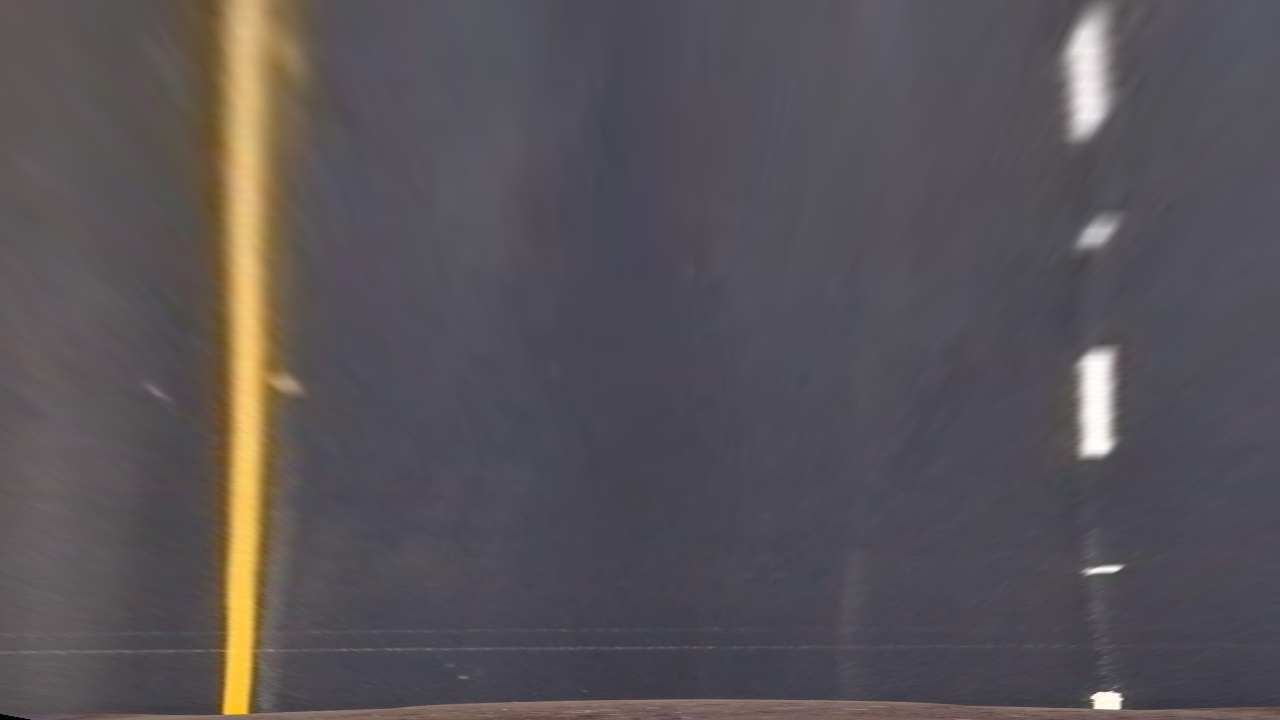
\includegraphics[width=0.8\linewidth]{warped_straightlines}
	\caption{Warped Straight Lines}
	\label{fig:warpedstraightlines}
\end{figure}




\noindent\rule{12.5cm}{0.5pt}




\subsection{Color transforms and gradients}%
\label{sub:color_transforms_and_gradients}


Then, with the warped image at hand, I used a combination of color and gradient thresholds. The code is in the function \texttt{color\_pipeline}.


I figure out that when the road is clear, the s\_channel is better to find the lanes but when the road is dark because of some shadow caused by the threes, the l\_channel was better. 

Because of that, I used a combination of l and s channel images with and without x gradient.

The result can be found in the Figure~\ref{fig:combined_binary}



\begin{figure}[htb!]
	\centering
	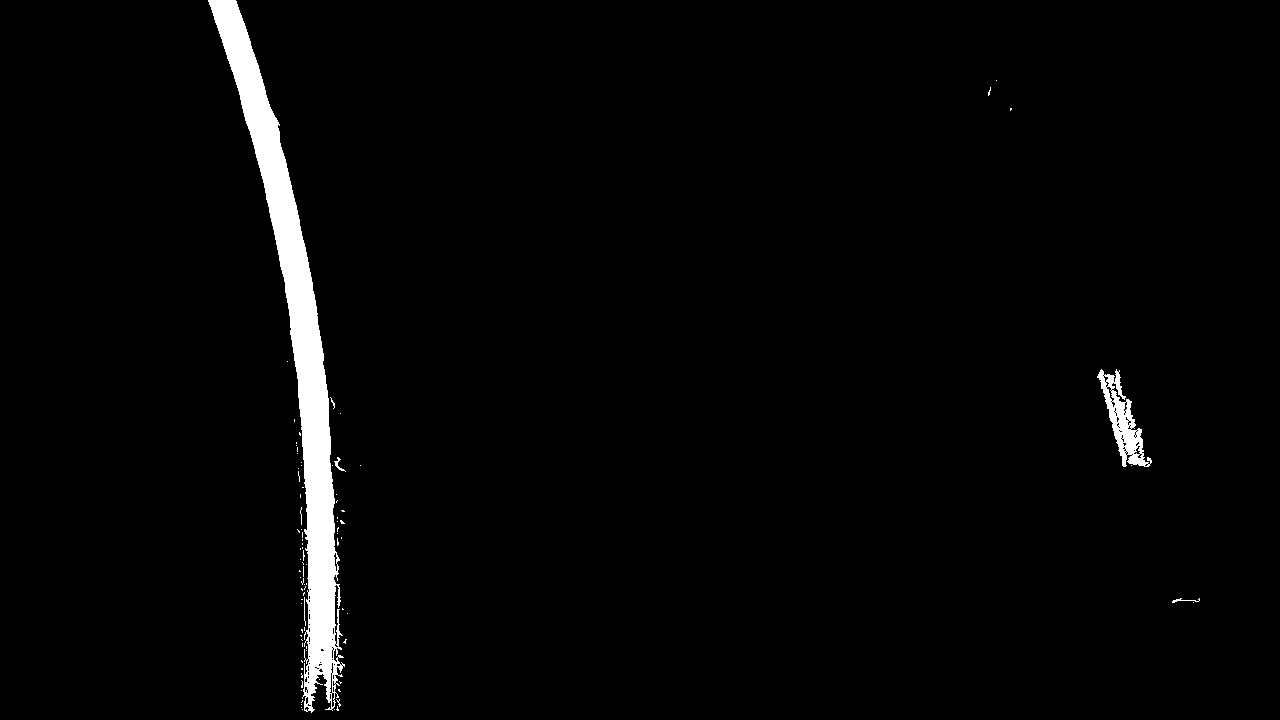
\includegraphics[width=0.8\linewidth]{combined_binary}
	\caption{Combined Binary}
	\label{fig:combined_binary}
\end{figure}




\subsection{Fitted Lane Lines}%
\label{sub:fitted_lane_lines}

The functions I used to fit the lines was \texttt{search\_around\_poly}. The result can be found in the Figure~\ref{fig:fitted_lines}.


For the video I used the \texttt{search\_around\_poly} but for illustration I used the \texttt{old\_search\_around\_poly} function to illustrate the windows. 

\begin{figure}[htb!]
	\centering
	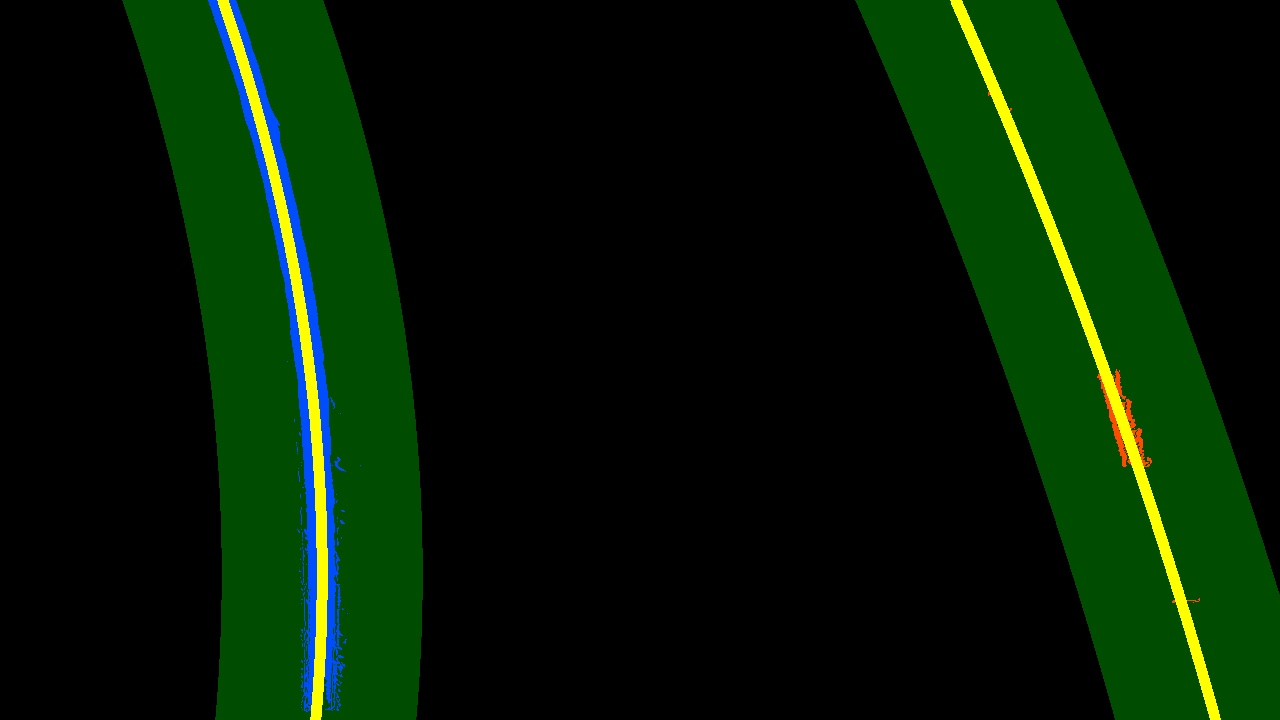
\includegraphics[width=0.8\linewidth]{fitted_lines}
	\caption{Fitted Lines}
	\label{fig:fitted_lines}
\end{figure}

\subsection{Curvature}%
\label{sub:curvature}

The curvature is being measured in the function \texttt{measure\_curvature\_real}. The useful pixels of the images were taken from the warped image so I endup with:

\begin{itemize}
	\item \texttt{ym\_per\_pix} = 30 / 720
	\item \texttt{xm\_per\_pix} = 3.7 / 900
\end{itemize}

The location of the vehicle was taken from the fitted lines. I computed the distance from the left line to the center of warped image. Also, I calculated the distance from the middle of the warped image to the right line. If the difference between this to values is greater than zero, the vehicle is on the left and if the difference is less than zero, the vehicle is on the right.



The final output is in the Figure~\ref{fig:output}

\begin{figure}[htb!]
	\centering
	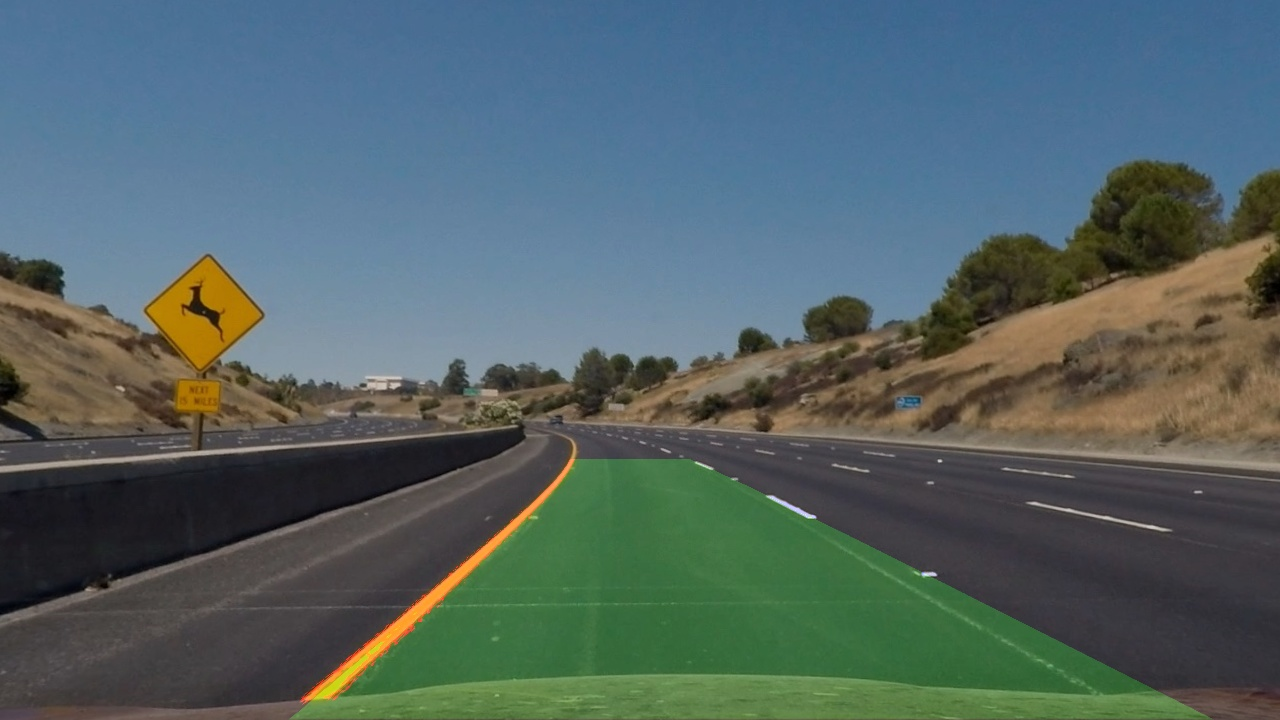
\includegraphics[width=0.8\linewidth]{output}
	\caption{output}
	\label{fig:output}
\end{figure}


Here's a \href{https://github.com/SamuelNavarro/SelfDriving/tree/master/AdvancedLaneFinding/Project/test_videos_output}{to the output video}






\section{Discussion}
\label{sec:discussion}



\begin{itemize}
	\item One of the problems I encounter was the fact that you have a difference in the frames when you are trying to diagnose the problems. It seems obvious when you know you are dealing with the undistorted frames but at the beginning I was trying to diagnose the problems with the original frame but applying the functions into the undistorted images.
	\item As in the previous project, I would like to implement this in C++ and check what are the differences.
	\item Another thing I could do to improve the pipeline is to compute the Exponential Moving Average of the fitted lines to give more weight to the recent frames and to update the lines based on the EWMA of the lines.
	\item Also, I wanted to provide a video with 4 different frames with the different process being showed in the video but I didn't have enough time.
\end{itemize}







\end{document}
